\chapter{RESULT AND ANALYSIS}
The result of the seminar report is to analysis word embedding models based on news classification. For getting the result, number of pre-processing tasks is performed which is explained in the following section.
\section{Preprocessing}
After data collection process is completed, this is not directly supplied into machine learning algorithm so, some preprocessing tasks need to be performed such as removing stop word, special character and identifying most frequent word etc. The sample of raw news is shown in the figure \ref{fig: Raw_dataset}.
\begin{figure}[H]
	\centering 
	\vspace{20pt}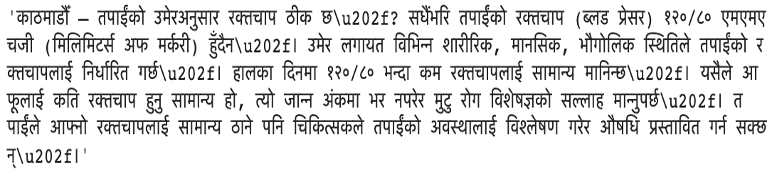
\includegraphics[width=10cm]{images/preprocessing1.png}
	\caption{Sample of Raw Dataset} 
	\label{fig: Raw_dataset}
\end{figure}
Stop words are removed by using the list of stop-words available in NLTK library. Additionally, some special characters are also removed from the raw dataset. All in all, stemming and lemmatization is not performed with these raw datasets. Dataset after completing preprocess is shown in the given figure \ref{fig:Processed_dataset}.
\begin{figure}[H] 
	\centering 
	\vspace{20pt}
\includegraphics[width=10cm]{images/preprocessing2.png}
	\caption{Sample Preprocess Dataset} 
	\label{fig:Processed_dataset}
	
\end{figure}
\section{Time Performance Analysis}
After the preprocessing task is completed, both Word2vec and ELMO modules are run with varying hyperparameter for the comparative analysis. Additionally, the time stamp required for training each of the models is captured. 
\subsection{Word2Vec}
Here Word2vec model is trained with the processed data for fixed number of features and window size but having different minimum count values. By this analysis it is concluded that this model is trained comparatively fast for minimum count 3 as compared to others. The calculated data are tabulated in the table \ref{table:Word2Vec_minimum_count}
\begin{center}
\begin{table}[H]
\caption{Time Taken by Word2Vec for different minimum count}
\label{table:Word2Vec_minimum_count}
\centering
\begin{tabular}{ |p{4cm}|p{2cm}|p{2cm}|p{2cm}|p{2cm}|  }
 \hline
 Number of Features & 200 &200 &200 &200  \\
 \hline
 Minimum Count   & 1 &2 &3 &4    \\
 \hline
 Window Size &5 &5 &5 &5 \\
 \hline
 Training Time(Second) &77 &59 &49 &50 \\
 \hline
\end{tabular}
\end{table}
\end{center}
The above calculation is visualized in the form of line graph, and which is displayed in the figure \ref{fig:fixed_window_word2vec}.
\begin{figure}[H]
	\centering 
	\vspace{20pt}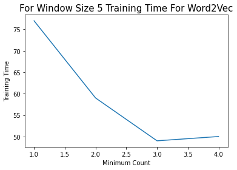
\includegraphics[width=10cm]{images/Word2Vec_fixed_window_line.png}
	\caption{For fixed window size training time for Word2Vec} 
	\label{fig:fixed_window_word2vec}
\end{figure}
Now, here train the same model with same training dataset for various window size, Training time is unexpectedly raised while expanding the window size. The numerical estimates are tabulated in table \ref{table:Minimum_word_word2vec} .
\begin{center}
\begin{table}[H]
\caption{For Fixed Minimum Count Training time for Word2Vec}
\label{table:Minimum_word_word2vec}
\centering
\begin{tabular}{ |p{4cm}|p{2cm}|p{2cm}|p{2cm}|p{2cm}|  }
 \hline
 Number of Features & 200 &200 &200 &200  \\
 \hline
 Minimum Count   & 1 &1 &1 &1    \\
 \hline
 Window Size &4 &8 &10 &12 \\
 \hline
 Training Time(Second) &67 &113 &133 &153 \\
 \hline
\end{tabular}
\end{table}
\end{center}
\subsection{ELMo}
Here ELMO model is trained with the processed data for fixed number of features. By this analysis it is concluded that this model takes longer time for training as compared to Word2Vec. This model takes 1 hours and 36 minutes for generating word embedding vector of preprocessing data. The calculation is depicted in the table \ref{table:training_time_for_ELMO} below.
\begin{center}
\begin{table}[H]
\caption{Training time for ELMO}
\label{table:training_time_for_ELMO}
\centering
\begin{tabular}{ |p{4cm}|p{6cm}|  }
 \hline
 Number of Features & 200 \\
 \hline
 Training Time  & 1 hour 36 minutes    \\
 \hline
\end{tabular}
\end{table}
\end{center}
\section{Model Evaluation}
\subsection{SVM}
For Word2Vec performance of the SVM model is remained constant while increasing the window size. Additionally, it gives maximum of 68 test accuracy for window size equal to eight. Different window size’s values are tabulated in the table \ref{table:SVM_model_accuracy_diff_window_size}.
\begin{center}
\begin{table}[H]
\caption{SVM Model Accuracy for Word2vec with Different Window Size}
\label{table:SVM_model_accuracy_diff_window_size}
\centering
\begin{tabular}{ |p{4cm}|p{2cm}|p{2cm}|p{2cm}|p{2cm}|  }
 \hline
 Number of Features & 200 &200 &200 &200  \\
 \hline
 Minimum Count   & 1 &1 &1 &1    \\
 \hline
 Window Size &4 &8 &10 &12 \\
 \hline
 Model Accuracy &67 &68 &68 &68 \\
 \hline
\end{tabular}
\end{table}
\end{center}
The above calculation is visualized in the form of bar graph and which is displayed in the figure \ref{fig:bargraph_SVM_model_accuracy_diff_window_size}.
\begin{figure}[H]
	\centering 
	\vspace{20pt}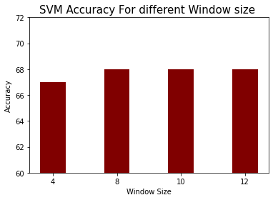
\includegraphics[width=10cm]{images/SVM_accuracy_for_different_window.png}
	\caption{SVM Model Accuracy for Word2vec with Different Window Size} 
	\label{fig:bargraph_SVM_model_accuracy_diff_window_size}
\end{figure}
Here Support Vector Machine Learning algorithm again train with the same dataset for various minimum count. This model showing slight fluctuation behavior while increasing the minimum count to 2,3,4 and so on. This model gives the highest of 67 percent test accuracy on odd number of minimum counts in our sample count. Finally, different test accuracy on different minimum count is tabulated in the table \ref{table: SVM_model_accuracy_diff_minimum_count}.
\begin{center}
\begin{table}[H]
\caption{SVM Model Accuracy for Word2vec with Different Minimum Count}
\label{table: SVM_model_accuracy_diff_minimum_count}
\centering
\begin{tabular}{ |p{4cm}|p{2cm}|p{2cm}|p{2cm}|p{2cm}|  }
 \hline
 Number of Features & 200 &200 &200 &200  \\
 \hline
 Minimum Count   & 2 &3 &4 &5    \\
 \hline
 Window Size &8 &8 &8 &8 \\
 \hline
 Model Accuracy &67 &66 &67 &66 \\
 \hline
\end{tabular}
\end{table}
\end{center}
The above calculation is visualized in the form of bar graph and which is displayed in the figure \ref{fig:bargraph_SVM_model_accuracy_diff_minimum_count}.

\begin{figure}[H]
	\centering 
	\vspace{20pt}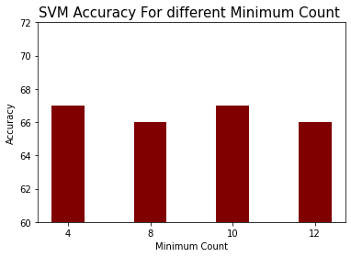
\includegraphics[width=10cm]{images/SVM_accuracy_for_different_minimum_count.png}
	\caption{SVM Model Accuracy for Word2vec with Different Minimum Count} 
	\label{fig:bargraph_SVM_model_accuracy_diff_minimum_count}
\end{figure}
In this seminar report ELMo Word embedding model is also used for the analysis. Because of insufficient of the computational resources, this model is only trained by taking features size of 20. Support Vector Machine learning algorithm gives similar accuracy of 67 percent for the ELMo vectorization as compared to Word2Vec. The detailed classification report of SVM by using ELMO word embedding is shown in the figure \ref{fig:SVM_classification_ELMo}.
\begin{figure}[H]
	\centering 
	\vspace{20pt}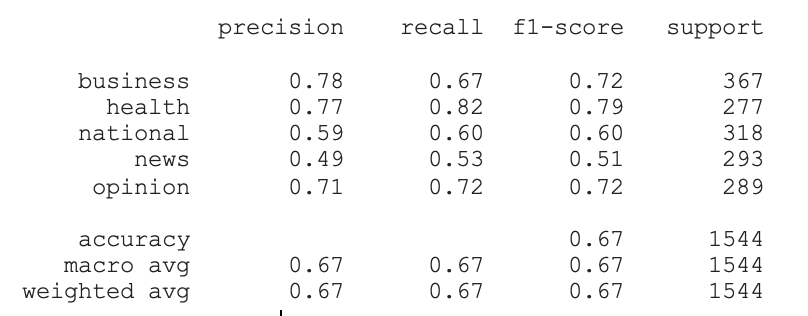
\includegraphics[width=10cm]{images/ELMO_for_SVM.png}
	\caption{SVM Classification Report for ELMO Word embedding} 
	\label{fig:SVM_classification_ELMo}
\end{figure}

\subsection{Random Forest}
For Word2Vec performance of the Random Forest model is increased slightly as compared to the SVM model. For taking 200 features and a single count this model gives the highest of 73 percent test accuracy on window size 4. The data are presented in the table \ref{table:Random_forest_word2vec_diff_window_size}.
\begin{center}
\begin{table}[H]
\caption{Random Forest Model Accuracy for Word2vec with Different Window Size}
\label{table:Random_forest_word2vec_diff_window_size}
\centering
\begin{tabular}{ |p{4cm}|p{2cm}|p{2cm}|p{2cm}|p{2cm}|  }
 \hline
 Number of Features & 200 &200 &200 &200  \\
 \hline
 Minimum Count   & 1 &1 &1 &1    \\
 \hline
 Window Size &4 &8 &10 &12 \\
 \hline
 Model Accuracy &73 &70 &70 &71 \\
 \hline
\end{tabular}
\end{table}
\end{center}
The above calculation is converted into the form of  bar graph which is depicted in the \ref{fig:Randomforest_acccuracy_different_windowsize}.
\begin{figure}[H]
	\centering 
	\vspace{20pt}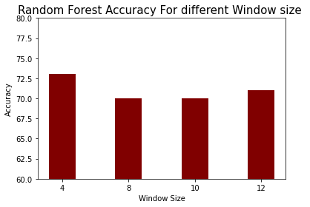
\includegraphics[width=10cm]{images/Randomforest_acccuracy_different_windowsize.png}
	\caption{Random Forest Model Accuracy for Word2vec with Different Window Size} 
	\label{fig:Randomforest_acccuracy_different_windowsize}
\end{figure}
For varying number of minimum counts and constant number of features and window size. The model accuracy is plummeted noticeably. Finally, different test accuracy on different minimum count is tabulated in the table \ref{table:SVM_model_different_minimum_count}.
\begin{center}
\begin{table}[H]
\caption{SVM Model Accuracy for Word2vec with Different Minimum Count}
\label{table:SVM_model_different_minimum_count}
\centering
\begin{tabular}{ |p{4cm}|p{2cm}|p{2cm}|p{2cm}|p{2cm}|  }
 \hline
 Number of Features & 200 &200 &200 &200  \\
 \hline
 Minimum Count   & 1 &2 &3 &4    \\
 \hline
 Window Size &4 &4 &4 &4 \\
 \hline
 Model Accuracy &73 &71 &71 &71 \\
 \hline
\end{tabular}
\end{table}
\end{center}
The above calculation is depicted in the figure .
\begin{figure}[H]
	\centering 
	\vspace{20pt}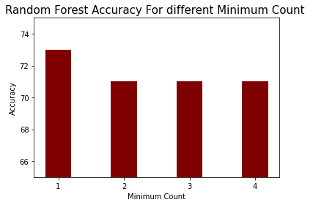
\includegraphics[width=10cm]{images/Random_forest_accuracy_for_different_minimum_count.png}
	\caption{Random Forest Model Accuracy for Word2vec with Different Window Size} 
	
\end{figure}
The word embedding value generated by the ELMO is also used for training the random forest machine learning algorithm. For this embedding random forest gives slightly higher accuracy as compared to the ELMO, it secures 74 percent test accuracy for the news classification system. All in all, classification report is shown in the figure \ref{fig:Random_forest_for_ELMo}.
\begin{figure}[H]
	\centering 
	\vspace{20pt}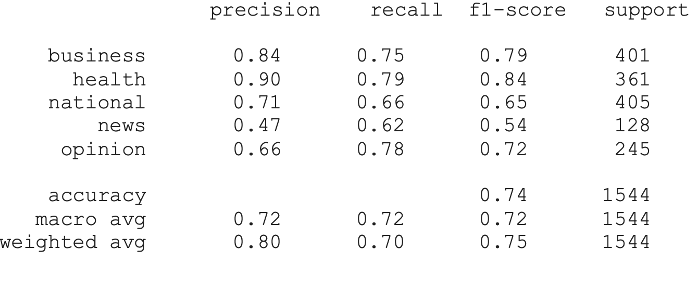
\includegraphics[width=10cm]{images/Random_forest_for_ELMO.png}
	\caption{Random Forest Classification Report for ELMO Word embedding} 
	\label{fig:Random_forest_for_ELMo}
\end{figure}
